%%%%%%%%%%%%%%%%%%%%%%%%%%%%%%%%%%%%%%%%%%%%%%%%%%%%%%%%%%%%%%%%%%%%%%%%%%%%%%%%
% Template for USENIX papers.
%
% History:
%
% - TEMPLATE for Usenix papers, specifically to meet requirements of
%   USENIX '05. originally a template for producing IEEE-format
%   articles using LaTeX. written by Matthew Ward, CS Department,
%   Worcester Polytechnic Institute. adapted by David Beazley for his
%   excellent SWIG paper in Proceedings, Tcl 96. turned into a
%   smartass generic template by De Clarke, with thanks to both the
%   above pioneers. Use at your own risk. Complaints to /dev/null.
%   Make it two column with no page numbering, default is 10 point.
%
% - Munged by Fred Douglis <douglis@research.att.com> 10/97 to
%   separate the .sty file from the LaTeX source template, so that
%   people can more easily include the .sty file into an existing
%   document. Also changed to more closely follow the style guidelines
%   as represented by the Word sample file.
%
% - Note that since 2010, USENIX does not require endnotes. If you
%   want foot of page notes, don't include the endnotes package in the
%   usepackage command, below.
% - This version uses the latex2e styles, not the very ancient 2.09
%   stuff.
%
% - Updated July 2018: Text block size changed from 6.5" to 7"
%
% - Updated Dec 2018 for ATC'19:
%
%   * Revised text to pass HotCRP's auto-formatting check, with
%     hotcrp.settings.submission_form.body_font_size=10pt, and
%     hotcrp.settings.submission_form.line_height=12pt
%
%   * Switched from \endnote-s to \footnote-s to match Usenix's policy.
%
%   * \section* => \begin{abstract} ... \end{abstract}
%
%   * Make template self-contained in terms of bibtex entires, to allow
%     this file to be compiled. (And changing refs style to 'plain'.)
%
%   * Make template self-contained in terms of figures, to
%     allow this file to be compiled. 
%
%   * Added packages for hyperref, embedding fonts, and improving
%     appearance.
%   
%   * Removed outdated text.
%
%%%%%%%%%%%%%%%%%%%%%%%%%%%%%%%%%%%%%%%%%%%%%%%%%%%%%%%%%%%%%%%%%%%%%%%%%%%%%%%%

\documentclass[letterpaper,twocolumn,10pt]{article}
\usepackage{usenix2019_v3}

% to be able to draw some self-contained figs
\usepackage{tikz}
\usepackage{amsmath}
\usepackage{graphicx}
\usepackage{filecontents}
\usepackage{xspace}
\usepackage{color, soul}
\usepackage{multirow}
\usepackage{hyperref}
\urlstyle{same}
\usepackage{subfigure}
\usepackage{subcaption}

\newcommand{\note}[1]{{\color{red}{\textbf{#1}}}}
\newcommand{\comment}[1]{{}}
\newcommand*\circled[1]{\tikz[baseline=(char.base)]{
            \node[shape=circle,fill,inner sep=0.4pt] (char) {\textcolor{white}{#1}};}}

\def\tick{\tikz\fill[scale=0.4](0,.35) -- (.25,0) -- (1,.7) -- (.25,.15) -- cycle;} 
\newcommand\ChangeRT[1]{\noalign{\hrule height #1}}

%-------------------------------------------------------------------------------
\begin{document}
%-------------------------------------------------------------------------------

%don't want date printed
\date{}

% make title bold and 14 pt font (Latex default is non-bold, 16 pt)
\title{\Large \bf Analysis of Server Throughput For Managed Big Data Analytics
    Workloads.}
}

%Overcoming the \note{M}emory \note{B}ound of Big
%Data Analytics to \note{I}mprove \note{S}erver \note{T}hroughput
%\note{U}sing \note{F}ast \note{S}torage Devices 

%for single author (just remove % characters)
\author{
{\rm Emmanouil Anagnostakis}\\
Institute of Computer Science (ICS), Foundation of Research and Technology -- Hellas (FORTH), Greece \\
Computer Science Department, University of Crete, Greece
}
%\and
%{\rm Second Name}\\
%Second Institution
% copy the following lines to add more authors
% \and
% {\rm Name}\\
%Name Institution
%} % end author

\maketitle
\begin{abstract}
    Nowadays datacenters experience problems with scaling their DRAM
    capacity.  \note{jk: please rewrite this sentence - is very
    complex.} This limitation causes big data analytics frameworks,
    which run on top of the Java Virtual Machine (JVM), to experience
    lack of sufficient memory. The lack of sufficient memory leads to
    long garbage collection (GC) cycles during the data processing.
    \note{jk: Say that they use more memory to reduce this overhead
    and then conclude with the last sentence}
    This overhead prevents the frameworks from effectively utilizing
    the CPU thus leading to low server throughput.

    In this paper, we conduct an analysis of server throughput for
    managed big data analytics frameworks when offloading the heap to
    fast storage devices. More specifically, we examine, whether
    storing data to fast storage devices instead of the main memory
    can help increase the throughput of the system by reducing memory
    pressure. \note{jk: we need to do make the term throughput more
    specific. E.g. Increase the CPU utilization} 
    We use a system called TeraHeap that moves objects from
    the Java managed heap to a secondary heap over a fast storage
    device to reduce the Garbage Collection overhead. We examine
    whether reducing the Java Garbage Collection overhead leads to
    more effective utilization of the available CPU by the
    application. Our primary focus is to analyze the system's
    performance under the colocation of multiple memory-bound
    instances.   Furthermore, we present a detailed methodology for
    running Apache Spark and Giraph using TeraHeap. The methodology
    includes conducting a research about the memory needs, i.e. Java
    Heap and IO Cache, of different big data analytics workloads when
    using Spark-Giraph with native JVM or JVM with TeraHeap.
    Understanding these needs helps us during the evaluation of
    running colocated instances.

    Our experimental results show that reducing Java Garbage
    Collection overhead by offloading the heap to fast storage devices
    significantly improves server throughput by up to 66\% against
    native Spark and Giraph. Finally, we also include a cost
    estimation to show that TeraHeap could reduce monetary cost by up
    to 50\% for running big data analytics, if deployed in a world
    cluster like Amazon's EC2 or Google Cloud Platform or Microsoft
    Azure Cloud, which are available to everyone.
\end{abstract}

\section{Introduction}
\label{sec:intro}

With the exponential growth of data in various fields such as
healthcare and social media, managed big data frameworks (e.g, Apache
Spark \cite{Spark} and Apache Giraph \cite{Giraph}) require large
amount of DRAM per core for data processing. During the processing, they generate large
amount of objects in the managed heap that span multiple computation
stages. The memory pressure that arises in the managed heap leads to
frequent garbage collection (GC) cycles. Frequent GCs waste CPU cycles 
and prevent application execution.

On the one hand, to reduce the frequency of GC and optimize performance, big data
frameworks offload objects from the managed heap to storage devices. However, these
objects need to be serialized to byte streams to be stored in the storage
device or to be deserialized into memory objects to be loaded back to memory. 
This practice leads to high serialization/deserialization overhead.
On the other hand infrastructure providers, trying to address the same problem increase memory per framework instance that runs in the server. This leaves CPU cores underutilized. 

Co-locating workloads aims to increase available resource utilization
thus increasing the throughput in server. 
In order to maximize throughput, the number of instances
increase to utilize all available DRAM. The result of this
practice is that the underlying machine runs out of memory, while the
 overhead of GC and S/D is still high. The remaining GC and S/D
overheads lead to the problem of wasting the CPU resources
to do unuseful work. This leads to the conclusion that the avalaible memory per core is
not enough for the Garbage Collector, S/D and the application.

The memory per core problem can better be understood when looking at
the resource usage and the characteristics of the servers of big
companies e.g. Alibaba and Facebook. When looking at the results of
Alibaba's traces analyses (\cite{Alibaba}, \cite{Alibaba1},
\cite{Alibabacolocated}) we see that memory usage is at an average of
80\%, while CPU usage stays at 40\%. This trace clearly shows that
DRAM utilization is high, while the CPU is under-utilized. In
Facebook's Twine presentation \cite{Twine}, they used a cluster of
machines where each machine had 40 cores and 80 GB DRAM. This means
that ratio of GB for memory per core was 2. The same ratio is shown in Facebook's Yosemite
\cite{Yosemite}. This shows that memory
capacity for each core is low while DRAM usage is high compared to the CPU usage. Most of the time many the CPU cores are
going to be idle because a few of them will be enough to carry out the
work.

To address the problem of DRAM capacity limitation, recent work
proposed solutions that extend the managed heaps over local flash
storage devices (e.g., NVMe SSD) or remote memory. On the one hand,
TMO \cite{TMO} offloads cold memory to fast storage devices using
a memory scheduling mechanism. On the other hand, CFM \cite{CFM}
utilizes remote DRAM as swap memory in order to increase total memory capacity
and reduce memory pressure. Of both works, only CFM shows
evaluation against managed big data analytics frameworks. However, this evaluation
includes only one Spark workload and is not focused on analytics.

This paper provides a methodological analysis of server throughput 
focused on managed big data analytics frameworks.
We investigate the off-heap direction of offloading the objects from the
managed heap to fast storage devices.
Specifically, we use TeraHeap (TH) \cite{TeraHeap}, a secondary managed
memory-mapped heap over an NVMe storage device, which is used to hold
the long lived objects instead of the main managed Java Heap. TeraHeap
1) eliminates Serialization/Deserialization overheads posed by this
kind of frameworks when moving data off-heap to/from fast storage
devices 2) reduces GC pauses drastically over the secondary heap. By
using TeraHeap, we aim to investigate the impact of reducing GC and S/D
to server throughput under workload co-location compared to Native Spark
and Giraph. We divide all the available DRAM
in our machine to 2,4 and 8 even budgets to run the co-located instances.
First we run each instance isolated to analyze performance and be able to study the interference when adding more
co-located instances. We run each individual workload with a different Spark or Giraph instance in a cgroup.
We do this to limit the memory budget for each instance. Memory budget is
the summary of Java Heap, IO Cache (Linux Page Cache) and JVM native memory. We choose
the Java Heap (H1) ratio over the total DRAM budget based on RedHat's decisions
for running containers as a baseline. We also run experiment with more Page Cache (PC) ratio than H1
to investigate Page Cache affection to the performance. We show performance of both Native Spark-Giraph and Spark-Giraph with TH in 3 different
memory per core scenarios, 4 GB per core, which is the current trend and 8 and 16 GB per core 
as possible future trends. We evaluate both offloading techniques by running 2 widely used
managed big data frameworks, Apache Spark and Giraph. We
specificaly run 4 different workloads with Spark with 4 and 8 GB per core.
We run 2 different workloads with Giraph with 8 and 16 GB per core.
We compare TeraHeap with the native Spark and Giraph distributions under workload
co-location and analyze their performance using several metrics like
GC, S/D, I/O and CPU utilization. Finally, we estimate the cost of running these
experiments in public world clusters like Amazon EC2, Google Cloud Platform (GCP)
and Microsoft Azure Cloud to see possible benefits of either of the two techniques.

Our experimental results show that there is indeed a problem with memory per core ratio
for managed big data frameworks.
A solution is to move the managed heap over fast storage devices to avoid both GC and S/D like TeraHeap and Panthera \cite{Panthera}.
Our experimental results show that reducing GC and S/D by offloading the heap to fast storage devices improves effective CPU utlization for Spark and also leaves place to run more co-located instances in the server for both frameworks.
Finally, we also include a cost estimation to show that reducing GC and S/D could reduce monetary cost by up to 50\% for running big data
analytics, in a world cluster like EC2, GCP or Microsoft Azure Cloud, which are available to
the public.

To summarize, this paper makes the following contributions: 
\begin{itemize}
    \item{A detailed methodology for running co-located Apache Spark and Giraph
        workloads with or without TeraHeap. 
	We show how to pick the DRAM budget for each co-located instance and how to divide this budget
		for the different memory needs of a group of processes.
		}

    \item{A comprehensive evaluation using the above methodology.
	    We run 4 Spark and 2 Giraph workloads in 3 memory per core scenarios
	    analyzing different aspects of performance like GC, S/D, I/O, average throughput, CPU utilization and CPU cycles. We show the interference impact of running multiple co-located managed big data frameworks workloads and show that reducing GC and S/D increases application throughput and utilizes the CPU in a better and more efficient way for Spark. We also show that decreasing GC and S/D, increases the number of co-located instances that can execute in the server.}

    \item{A cost estimation of running our experiments in real-world
        cloud platforms like Amazon EC2, Google Cloud and Microsoft
        Azure.}
\end{itemize}

\section{Related Work}

We group the related work in the two following categories:
\begin{itemize}
\item{Works that examine collocation of workloads}
\item{Other analyses on managed big data frameworks}
\end{itemize}

\subsection{Work that examine the collocation of workloads}
To our best knowledge there is limited work in investigating workload co-location. Here we refer to some works does in this area.

Baig et al. in \cite{NUMA} investigate how Spark-based workloads are impacted by the effects of NUMA-placement decisions. This is something we do not do in our work, because we run our experiments in a single NUMA island to avoid NUMA effects that could complicate the understanding of GC, S/D and the aspects of execution that we investigate. Apart from that difference they investigate the performance of co-located spark workers where each worker runs in a different NUMA island. They count remote memory accesses and context switches in CPU. Chen et al. in \cite{interference} analyze the characteristics of co-located workloads running in containers on the same server from the perspective of hardware events. These events include inctructions per cycle, branch prediction misses and dTLB misses. They also show the execution time of co-located workloads, but they do not provide further analysis or breakdown.

\subsection{Other analyses on managed big data frameworks}

Here we refer to other evaluation works targetting managed big data frameworks.
These works do not provide analyses for workload co-location.

Jiang et al. in \cite{inmem} study the behavior of Spark Workloads in comparison to those of Giraph, CloudSuite, SPEC CPU2006,
TPC-C, and DesktopCloud on system (i.e. disk utilization, memory bandwidth)  and microarchitectural level (instructions per cycle). This work
also provides an analysis for Spark and Giraph examining the behaviour from a different scope than ours. However, it does not provide a breakdown to the execution time of the workloads (i.e. GC, S/D) or CPU utilization analysis.
Ousterhout et al. \cite{makingsense} provide a methodology based on dynamic logging and profiling for quantifying performance bottlenecks in distributed computation frameworks, and use it to analyze the Spark’s performance. They refer and measure S/D, GC and CPU utilization but they don't refer to co-located workloads or target other frameworks. Batarfi et al. \cite{giraphgraphalytics} analyze the performance of many graph processing frameworks including Giraph. They provide results on RAM usage, CPU utilization and execution time. However, they investigate a different aspect from execution time. They break it down to the time taken by each phase of the workload execution.  They also only show results for graph processing and do not target other areas like machine learning as we do. Furthermore, their work is evaluated only aganst Spark. 


\section{Experimental Methodology}
\label{sec:method}

In this section we discuss our methodological decisions.

Our methodology answers the following questions:
\begin{itemize}
	\item{What workloads did we choose to run for our experiments and why?}
	\item{How do we investigate the memory per core problem?}
	\item{How do we choose the configurations for running the co-located experiments?}
	\item{How do we decide what percentage of total cgroup DRAM to use for Java Heap for each cgroup?}
	\item{Is cost a contributing factor to pursuing higher throughput for a server?}
\end{itemize}

\subsection{Workloads}
For our experiments with Spark, we selected four specific workloads from two
different categories of the Spark Bench suite \cite{Spark-Bench}: Page Rank (PR) and Connected
Component (CC) from GraphX \cite{GraphX} and Linear Regression (LinR) and Logistic Regression (LogR)
from MLLib \cite{MLLib}. For Giraph we choose PageRank and Community detection 
using label propagation (CDLP) from LDBC Graphalytics \cite{ldbc}. The primary reason for selecting these workloads for Spark is that
they represent different types of algorithms: PR and CC are graph-based workloads, while LinR and LogR are machine learning
workloads. Giraph is a graph processing framework so we only used graph workloads. All of these
workloads are well-established and commonly used for benchmarking big
data analytics systems, making them a suitable choice for our
experiments. Overall, the selection of these workloads allows us to
evaluate the performance of Spark and Giraph in a variety of contexts. Furthermore it allows us to
provide insights into the performance of both frameworks with or without using TeraHeap.


\subsubsection{PageRank}
PageRank is a widely used graph-based algorithm that measures the
importance of nodes in a network. It has become a popular benchmark
for evaluating the performance of distributed systems, including big
data analytics systems like Apache Spark and Giraph. PageRank is computationally
intensive and requires significant memory and I/O resources, making it
a suitable workload for evaluating performance of managed big data frameworks. Additionally, PageRank is a
common algorithm in real-world applications, such as search engines
and social networks, making it relevant for practical use cases.

\subsubsection{LinearRegression}
LinearRegression is a machine learning algorithm that is used to
predict numerical values based on input data. It is a well-known and
widely used algorithm in machine learning, and is commonly used for
regression analysis in fields such as economics, finance, and
engineering. LinearRegression is computationally intensive and
requires significant memory and I/O resources, making it a suitable
workload for evaluating the performance of managed big data frameworks.

\subsubsection{Logistic Regression}
LogisticRegression is a machine learning algorithm that is used to
model the probability of a binary or categorical outcome based on one
or more independent variables. It is commonly used in predictive
analytics to classify data based on historical data. In Spark-bench,
LogisticRegression is implemented as a machine learning workload,
where the dataset is represented as an RDD of feature vectors and
labels. The LogisticRegression workload involves training a logistic
regression model on the dataset, using an iterative optimization
algorithm such as gradient descent. The workload is computationally
intensive and requires a significant amount of memory to store the
dataset and model parameters, therefore a suitable choise for our experiments..

\subsubsection{Connected Component}
ConnectedComponent is a graph algorithm that is used to identify the
connected components of a graph. It is commonly used in social network
analysis to identify clusters of users with similar interests or
relationships. In Spark-bench, ConnectedComponent is implemented as a
graph processing workload, where the graph is represented as an RDD of
edges and vertices. The ConnectedComponent workload involves iterating
over the graph, identifying the connected components of each node, and
merging the components as necessary. The workload is computationally
intensive and requires a significant amount of memory to store the
graph, therefore a suitable choise for our experiments.

\subsubsection{Community Detection Label Propagation}
The Community Detection using Label Propagation (CDLP) workload, another key component of the Graphalytics benchmark, aims to identify communities within a graph based on label propagation techniques. The CDLP workload assigns labels to nodes iteratively, with each node adopting the most frequently occurring label among its neighbors. This iterative process propagates labels throughout the graph, eventually converging to stable communities. Community detection is a fundamental task in graph analysis, enabling researchers to uncover groups of nodes that exhibit strong internal connectivity. It has applications in social network analysis, recommendation systems, and anomaly detection. The CDLP workload in the Graphalytics benchmark provides a standardized evaluation of graph processing systems' performance in terms of community detection scalability, convergence, and accuracy. By benchmarking CDLP, researchers and practitioners can compare the efficiency and effectiveness of different graph processing platforms and algorithms for community detection tasks.

\subsection{Memory-per-core}

\begin{table}[thbp]
  \centering
  \caption{Configurations}
  \label{tab:setups}
  \begin{tabular}{|c|c|c|c|}
    \hline
	  \textbf{Workload} & \textbf{Framework} & \textbf{Dataset (GB)} & \textbf{DRAM GB / core} \\
    \hline
	  PR & Spark & 8 & 4 \\
	  LinR & Spark & 64 & 4 \\
	  LinR & Spark & 128 & 8 \\
    	LogR & Spark & 64 & 4 \\
	  CC & Spark & 8 & 4 \\
	  PR & Giraph & 13 & 4 \\
	  CDLP & Giraph & 13 & 4 \\
	  PR & Giraph & 13 & 8 \\
	  CDLP & Giraph & 13 & 8 \\
    \hline
  \end{tabular}
\end{table}


We investigate performance in two memory-per-core scenarios. Our main focus is 4 GB / core 
which is the next possible trend in datacenters based on \ref{sec:intro}. The other
is 8 GB / core which is a possible future trend. For the 4 GB / core scenario we use 64 GB memory with 16 cores.
In this setup, we run 4 workloads with Native Spark and Spark using TH and 2 workloads with Native Giraph and Giraph using TH. For the 8 GB / core scenario we run 1 workload with Native Spark and Spark using TeraHeap and 2 workloads with Native Giraph and Giraph using TeraHeap. We also choose 8 GB / core for Giraph because it experiences more memory pressure than Spark. This happens because it does not have
an aggresive memory offloading mechanism. For this setup we use 128 GB of memory with 16 cores. 
Table \ref{tab:setups} summarizes all setups with the coresponding workloads and datasets.

\subsection{Choosing the configurations to run the co-located experiments}
To utilize all the available DRAM of the machine we choose a simple method. 
We divide the total DRAM of the machine by the number of co-located workloads we run for each experiment.
For simplicity and time management we choose the numbers 1,2,4,8. However, there are 2 problems with that decision
than we need to overcome. The first is that we need a number that is exactly divided by these numbers to give the same amount of DRAM to
all cgroups. The second is that we need to leave memory to the OS for system tasks that are executed along with the system reserved memory of 2 GB. For the 4 GB memory/core scenario we utilize
56 GB out of 64 GB total DRAM and leave the rest 8 GB to the OS which is a safe option. For the 8 GB memory/core scenario we utilize
120 out of 128 GB total DRAM and leave the rest 8 GB to the OS. 
In both scenarios we choose the number closer to the total DRAM. After having perfomed these calculations we run each experiment isolated and break down the execution time to know how each experiment performs isolated. Then we run the co-located experiments and study the interference in execution. For the co-located experiments we run the same workload with the same dataset size for all instances. We do this for simplicity of explaining the results. For all experiments we have swap memory disabled.

\subsection{Cgroup DRAM percentage for Java Heap}
We use cgroups \cite{cgroups} to restrict the DRAM for all processes in a single instance of Spark and Giraph.
For cgroups we choose as a baseline an 80\% of total cgroup DRAM budget for H1 as RedHat does for its cgroups from June 2023 \cite{redhatblog}.
The rest 20\% remains to the OS to be used for Page Cache.
For TeraHeap we also run experiments with 40\% for H1 to investigate what happens when Page Cache dominates H1.
For Native Spark and Giraph we do not report results for those experiments because we saw that Page Cache makes no difference.

\subsection{Cost estimation}
Renting servers is a common practice for organizations requiring
computational resources, and the question arises as to whether
reducing the monetary cost is possible by achieving higher throughput
and faster workload completion. The relationship between cost
reduction and achieving higher throughput on rented servers is indeed
significant. By optimizing server performance, efficiently utilizing
resources, implementing workload scheduling, and improving
productivity, organizations can realize cost savings. Achieving higher
throughput and faster workload completion can lead to a reduced rental
duration, minimizing the time and associated costs of server usage.
Efficient resource utilization and workload scheduling contribute to
cost reduction by minimizing the number of servers required and
maximizing their utilization. Rental pricing models that take into
account resource utilization or data processed can further reduce
costs for organizations achieving higher throughput. Additionally,
improved productivity resulting from higher throughput and faster
workload completion enhances overall efficiency, allowing
organizations to accomplish more work within the same rental period
and reducing rental expenses. Therefore, pursuing higher throughput
and faster workload completion offers tangible benefits in terms of
monetary cost reduction for organizations renting servers. 

In order to estimate the cost of our evaluation in real-world public clusters we
chose a variety of providers like Amazon \cite{EC2}, Google \cite{GCP} and Microsoft \cite{Azure}. This
way we covered the most known providers and platforms someone would
choose to run their workloads on. We chose 2 machines from each
platform identical to the specifications of our 64 and 128 GB DRAM
machines. These are the cheapest machines of that particular category
offered by the platform. We then used the platform's pricing
calculator to estimate the cost of renting that machine for the time
needed for each configuration to finish execution of all instances. We noticed that the price for
renting the storage device is really amenable to the cost for renting the machine.

\section{Evaluation}
\label{sec:eval}

\begin{figure}[thbp]
\centering
    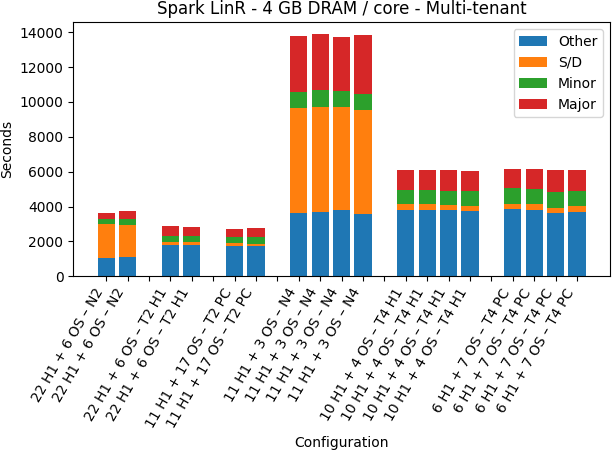
\includegraphics[width=\linewidth]{./fig/linr64.png}
    \caption{Execution time breakdown for multiple instances of
    LinearRegression using the 64 GB total DRAM setup. E.g.
    22-28-64-Native 1 indicates the first of the 2-4-8 instances that
    was run in parallel and uses 22 GB H1 - 28 GB total cgroup DRAM
    and 64 GB total DRAM for the machine.}
    \label{fig:linr64}
    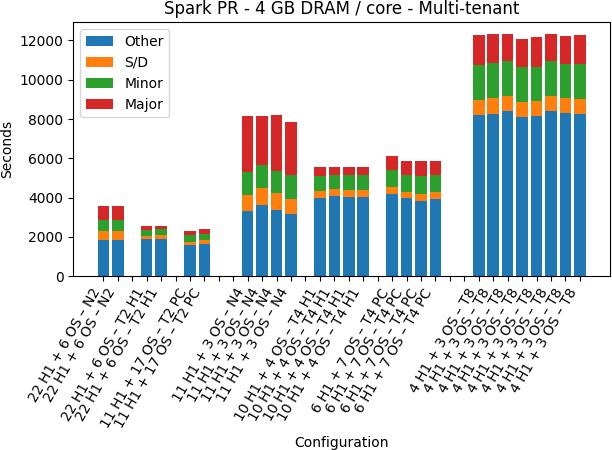
\includegraphics[width=\linewidth]{./fig/pr64.png}
    \caption{Execution time breakdown for multiple instances of
    PageRank using the 64 GB total DRAM setup. E.g. 22-28-64-Native 1
    indicates the first of the 2-4-8 instances that was run in
    parallel and uses 22 GB H1 - 28 GB total cgroup DRAM and 64 GB
    total DRAM for the machine.}
    \label{fig:pr64}
\end{figure}

\begin{figure}[thbp]
	\centering
    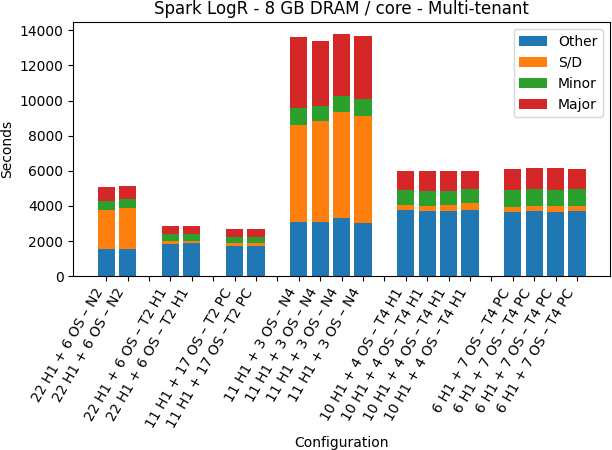
\includegraphics[width=\linewidth]{./fig/logr64.png}
    \caption{Execution time breakdown for multiple instances of
    Logistic Regression using the 64 GB total DRAM setup. E.g.
    22-28-64-Native 1 indicates the first of the 2-4-8 instances that
    was run in parallel and uses 22 GB H1 - 28 GB total cgroup DRAM
    and 64 GB total DRAM for the machine.}
    \label{fig:logr64}

    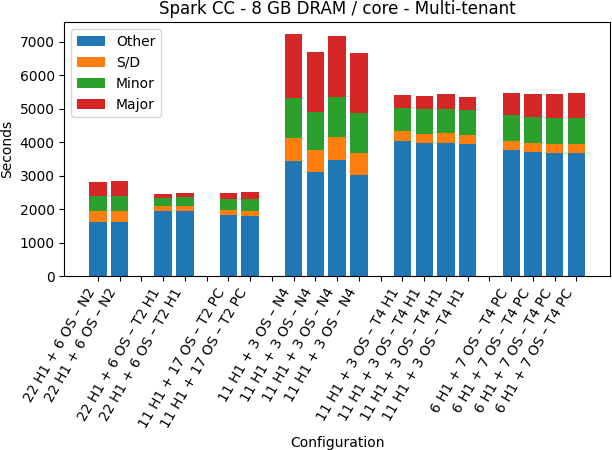
\includegraphics[width=\linewidth]{./fig/cc64.png}
    \caption{Execution time breakdown for multiple instances of
    Connected Component using the 64 GB total DRAM setup. E.g.
    22-28-64-Native 1 indicates the first of the 2-4-8 instances that
    was run in parallel and uses 22 GB H1 - 28 GB total cgroup DRAM
    and 64 GB total DRAM for the machine.}
    \label{fig:cc64}
\end{figure}

\begin{figure}[thbp]
	\centering
    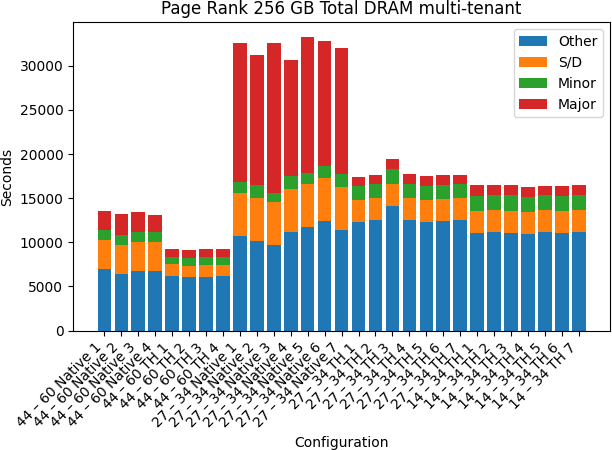
\includegraphics[width=\linewidth]{./fig/pr256.png}
    \caption{Execution time breakdown for multiple instances of
    PageRank using the 256 GB total DRAM setup. E.g. 44-60-256-Native
    1 indicates the first of the 2-4-8 instances that was run in
    parallel and uses 44 GB H1 - 60 GB total cgroup DRAM and 256 GB
    total DRAM for the machine.} 
    \label{fig:pr256}
    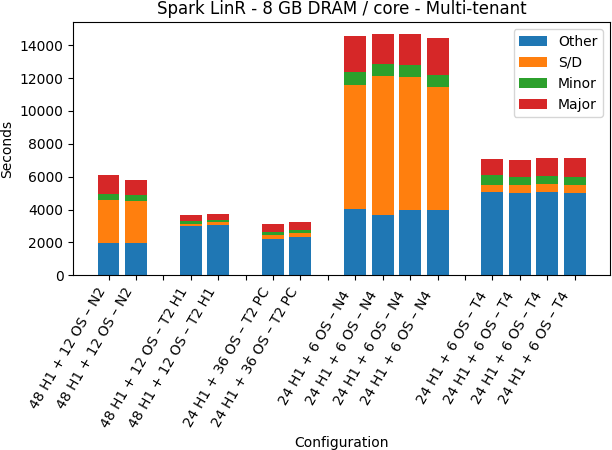
\includegraphics[width=\linewidth]{./fig/linr128.png}
    \caption{Execution time breakdown for multiple instances of
    LinearRegression using the 128 GB total DRAM setup. E.g.
    22-28-64-Native 1 indicates the first of the 2-4-8 instances that
    was run in parallel and uses 22 GB H1 - 28 GB total cgroup DRAM
    and 64 GB total DRAM for the machine.}
    \label{fig:linr128}
\end{figure}


\subsection{Experiments with colocated instances}

Here we look at the colocated experiments of Spark and Giraph.
We explain each figure from 2 aspects:
\begin{itemize}
\item{The differences in the time breakdown while number of instances increase for each configuration.}
\item{A comparison between the different configurations while instances increase.}
\end{itemize}

Figure \ref{fig:linr64} shows the performance of multiple
Native-TeraHeap Spark instances running LinearRegression with 64 GB
dataset per instance in our 64 GB DRAM machine. Each instance of Spark
uses one executor with 8 cores per executor. Available DRAM is 56 GB
and 8 GB are left to the Operating system, resulting in 64 GB total
DRAM. All configurations utilize 56 of 64 GB total DRAM. 
Starting from the left of the graph, the first 6 bars show the
performance of 3 runs. The first run is with 2 colocated Native Spark instances.
Another run with 2 colocated TH Spark instances with H1 dominating Page Cache
and a third run with 2 colocated TH Spark instances where Page Cache dominates H1. 
Each instance of the first 2 runs uses 22 GB DRAM for H1 (Java Heap) and 6 GB for rest of the services.
The third run uses 11 GB DRAM for H1 and 17 GB for Page Cache for each instance. 
The rest 12 bars show the performance of another 3 runs. The first run is with 4 colocated Native Spark instances.
Another run with 4 colocated TH Spark instances with H1 dominating Page Cache
and a third run with 4 colocated TH Spark instances where Page Cache dominates H1. 
Each instance of the first run uses 11 GB DRAM for H1 (Java Heap) and 3 GB for rest of the services. 
The second run uses 10 GB DRAM for H1 and 4 GB for Page Cache for each instance. 
The third run uses 6 GB DRAM for H1 and 8 GB for Page Cache for each instance. 
Considering the first aspect we see that GC and S/D increase dramatically for Native Spark along with significant increase to Other time. GC differences are witnessed because the heap capacity decreases and that causes memory pressure. TeraHeap Spark shows a slight increase to Major GC while the number of instances increases. This is because of the decreased heap capacity. Other time increases because more objects are moved to TeraHeap and read/write traffic increases but this is a good trade-off because all the GC is absorbed. S/D is completely absorbed by MMIO. From the third aspect, as instances increase in the server the benefit gap between Native and TeraHeap Spark becomes bigger. As Native Spark starves from more GC and S/D, TeraHeap maintains its benefits. 

Figure \ref{fig:pr64} shows the performance of multiple
Native-TeraHeap Spark instances running PageRank with 8 GB
dataset per instance in our 64 GB DRAM machine. Each instance of Spark
uses one executor with 8 cores per executor. Available DRAM is 56 GB
and 8 GB are left to the Operating system, resulting in 64 GB total
DRAM. All configurations utilize 56 of 64 GB total DRAM.
Starting from the left of the graph, the first 6 bars show the
performance of 3 runs. The first run is with 2 colocated Native Spark instances.
Another run with 2 colocated TH Spark instances with H1 dominating Page Cache
and a third run with 2 colocated TH Spark instances where Page Cache dominates H1.
Each instance of the first 2 runs uses 22 GB DRAM for H1 (Java Heap) and 6 GB for rest of the services.
The third run uses 11 GB DRAM for H1 and 17 GB for Page Cache for each instance. 
The next 12 bars show the performance of another 3 runs. The first run is with 4 colocated Native Spark instances.
Another run with 4 colocated TH Spark instances with H1 dominating Page Cache
and a third run with 4 colocated TH Spark instances where Page Cache dominates H1.
Each instance of the first run uses 11 GB DRAM for H1 (Java Heap) and 3 GB for rest of the services.
The second run uses 10 GB DRAM for H1 and 4 GB for Page Cache for each instance.
The third run uses 6 GB DRAM for H1 and 8 GB for Page Cache for each instance.
The last 8 bars refer to 8 colocated instances of TeraHeap Spark only. 
We were unable to decrease H1 enough to run 8 colocates instance of Native Spark
because JVM runs out of memory. Each instance of the run uses 4 GB DRAM for H1 (Java Heap) and 3 GB for Page Cache.
Considering the first aspect we see that Minor and Major GC increase dramatically for Native Spark along with significant increase to Other time. Minor and Major GC differences are witnessed because the heap capacity decreases and that causes memory pressure. TeraHeap Spark shows a slight increase to Major GC while the number of instances increases. This is because of the decreasing heap capacity. Other time increases because more objects are moved to TeraHeap but this is a good trade-off because all the GC is absorbed. S/D is completely absorbed by MMIO. From the second aspect, as instances increase in the server the benefit gap between Native and TeraHeap Spark becomes bigger. As Native Spark starves from more GC and S/D, TeraHeap maintains its benefits.

Figure \ref{fig:logr64} shows the performance of multiple
Native-TeraHeap Spark instances running Logistic Regression with 64 GB
dataset per instance in our 64 GB DRAM machine. Each instance of Spark
uses one executor with 8 cores per executor. Available DRAM is 56 GB
and 8 GB are left to the Operating system, resulting in 64 GB total
DRAM. All configurations utilize 56 of 64 GB total DRAM.
Starting from the left of the graph, the first 6 bars show the
performance of 3 runs. The first run is with 2 colocated Native Spark instances.
Another run with 2 colocated TH Spark instances with H1 dominating Page Cache
and a third run with 2 colocated TH Spark instances where Page Cache dominates H1.
Each instance of the first 2 runs uses 22 GB DRAM for H1 (Java Heap) and 6 GB for rest of the services.
The third run uses 11 GB DRAM for H1 and 17 GB for Page Cache for each instance. 
The next 12 bars show the performance of another 3 runs. The first run is with 4 colocated Native Spark instances.
Another run with 4 colocated TH Spark instances with H1 dominating Page Cache
and a third run with 4 colocated TH Spark instances where Page Cache dominates H1.
Each instance of the first run uses 11 GB DRAM for H1 (Java Heap) and 3 GB for rest of the services.
The second run uses 10 GB DRAM for H1 and 4 GB for Page Cache for each instance.
The third run uses 6 GB DRAM for H1 and 8 GB for Page Cache for each instance.
Considering the first aspect we see that GC and S/D increase dramatically for Native Spark along with significant increase to Other time. GC differences are witnessed because the heap capacity decreases and that causes memory pressure. TeraHeap Spark shows a slight increase to Major GC while the number of instances increases. This is because of the decreased heap capacity. Other time increases because more objects are moved to TeraHeap and read/write traffic increases but this is a good trade-off because all the GC is absorbed. S/D is completely absorbed by MMIO. From the third aspect, as instances increase in the server the benefit gap between Native and TeraHeap Spark becomes bigger. As Native Spark starves from more GC and S/D, TeraHeap maintains its benefits. 

Figure \ref{fig:cc64} shows the performance of multiple
Native-TeraHeap Spark instances running Connected Component with 8 GB
dataset per instance in our 64 GB DRAM machine. Each instance of Spark
uses one executor with 8 cores per executor. Available DRAM is 56 GB
and 8 GB are left to the Operating system, resulting in 64 GB total
DRAM. All configurations utilize 56 of 64 GB total DRAM.
Starting from the left of the graph, the first 6 bars show the
performance of 3 runs. The first run is with 2 colocated Native Spark instances.
Another run with 2 colocated TH Spark instances with H1 dominating Page Cache
and a third run with 2 colocated TH Spark instances where Page Cache dominates H1.
Each instance of the first 2 runs uses 22 GB DRAM for H1 (Java Heap) and 6 GB for rest of the services.
The third run uses 11 GB DRAM for H1 and 17 GB for Page Cache for each instance. 
The next 12 bars show the performance of another 3 runs. The first run is with 4 colocated Native Spark instances.
Another run with 4 colocated TH Spark instances with H1 dominating Page Cache
and a third run with 4 colocated TH Spark instances where Page Cache dominates H1.
Each instance of the first run uses 11 GB DRAM for H1 (Java Heap) and 3 GB for rest of the services.
The second run uses 10 GB DRAM for H1 and 4 GB for Page Cache for each instance.
The third run uses 6 GB DRAM for H1 and 8 GB for Page Cache for each instance.
Considering the first aspect we see that Minor and Major GC increase dramatically for Native Spark along with significant increase to Other time. Minor and Major GC differences are witnessed because the heap capacity decreases and that causes memory pressure. TeraHeap Spark shows a slight increase to Major GC while the number of instances increases. This is because of the decreasing heap capacity. Other time increases because more objects are moved to TeraHeap but this is a good trade-off because all the GC is absorbed. S/D is completely absorbed by MMIO. From the second aspect, as instances increase in the server the benefit gap between Native and TeraHeap Spark becomes bigger. As Native Spark starves from more GC and S/D, TeraHeap maintains its benefits.

Figure \ref{fig:pr256} shows the performance of multiple
Native-TeraHeap Spark instances running PageRank with 32 GB
dataset per instance in our 256 GB DRAM machine. Each instance of Spark
uses one executor with 8 cores per executor. Available DRAM is 240 GB
and 16 GB are left to the Operating system, resulting in 256 GB total
DRAM. All configurations utilize 240 of 256 GB total DRAM.
Starting from the left of the graph, the first 8 bars show the
performance of 2 runs. The first run is with 4 colocated Native Spark instances.
Another run with 4 colocated TH Spark instances with H1 dominating Page Cache.
Each instance of the first 8 runs uses 48 GB DRAM for H1 (Java Heap) and 12 GB for rest of the services including Page Cache.
The next 21 bars show the performance of another 3 runs. The first run is with 7 colocated Native Spark instances.
Another run with 7 colocated TH Spark instances with H1 dominating Page Cache
and a third run with 7 colocated TH Spark instances where Page Cache dominates H1.
Each instance of the first run uses 27 GB DRAM for H1 (Java Heap) and 7 GB for rest of the services.
The second run uses 27 GB DRAM for H1 and 7 GB for Page Cache for each TH instance.
The third run uses 14 GB DRAM for H1 and 20 GB for Page Cache for each TH instance.
Considering the first aspect we see that Minor and Major GC increase dramatically for Native Spark along with significant increase to Other time. Minor and Major GC differences are witnessed because the heap capacity decreases and that causes memory pressure. TeraHeap Spark shows a slight increase to Major GC while the number of instances increases. This is because of the decreasing heap capacity. Other time increases because more objects are moved to TeraHeap but this is a good trade-off because all the GC is absorbed. S/D is completely absorbed by MMIO. From the second aspect, as instances increase in the server the benefit gap between Native and TeraHeap Spark becomes bigger. As Native Spark starves from more GC and S/D, TeraHeap maintains its benefits.

\subsection{Is the CPU utilization of the server increasing
accordingly to throughput?}
\begin{figure}[thbp]
	\centering
        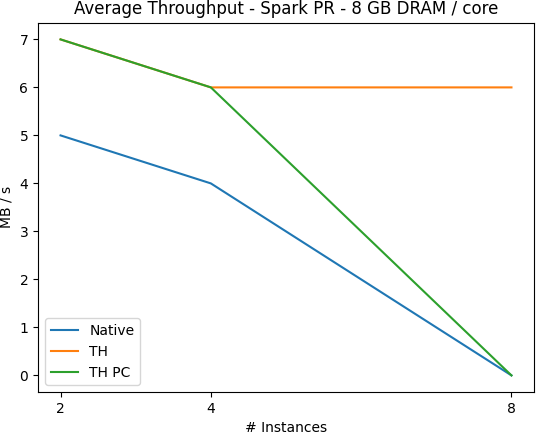
\includegraphics[width=\linewidth]{./fig/PR_64_THR.png}
    \caption{Page Rank 64 GB DRAM setup Native and TeraHeap throughput
    as the number of instances increases. Configurations starting with
    N denote a run with Native instances of Spark and with T with
    TeraHeap. H1 is a run with the memory budget configured to contain
    a bigger size for H1 than PageCache and PC the opposite. E.g. T2
    PC is a run of 2 concurrent TeraHeap instances with exactly the
    same configuration.}
\label{fig:pr_64_thr}
        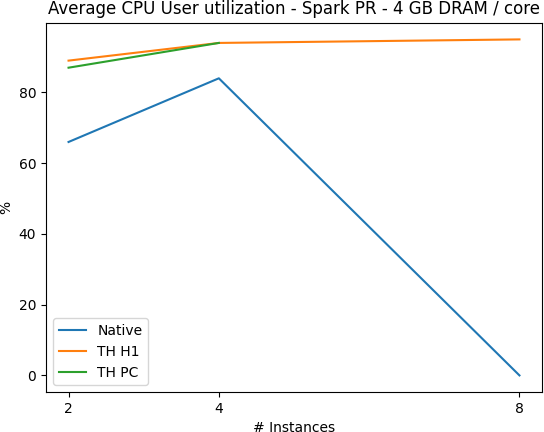
\includegraphics[width=\linewidth]{./fig/PR_64_USR.png}
    \caption{Page Rank 64 GB DRAM setup Native and TeraHeap User CPU utilization
    as the number of instances increases. Configurations starting with
    N denote a run with Native instances of Spark and with T with
    TeraHeap. H1 is a run with the memory budget configured to contain
    a bigger size for H1 than PageCache and PC the opposite. E.g. T2
    PC is a run of 2 concurrent TeraHeap instances with exactly the
    same configuration.}
		\label{fig:pr_64_usr}
\end{figure}

\begin{figure}[thbp]
	\centering
        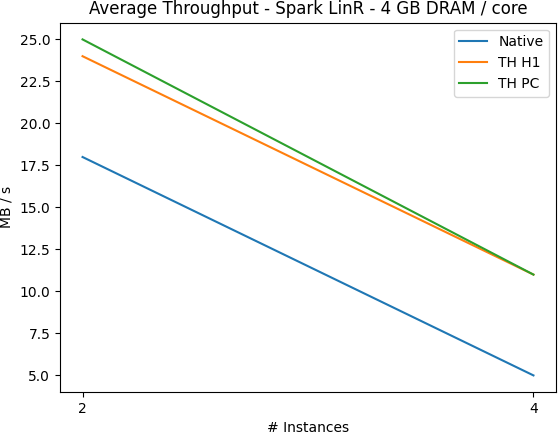
\includegraphics[width=\linewidth]{./fig/LINR_64_THR.png}
    \caption{Linear Regression 64 GB DRAM setup Native and TeraHeap
    throughput as the number of instances increases. Configurations
    starting with N denote a run with Native instances of Spark and
    with T with TeraHeap. H1 is a run with the memory budget
    configured to contain a bigger size for H1 than PageCache and PC
    the opposite. E.g. T2 PC is a run of 2 concurrent TeraHeap
    instances with exactly the same configuration.}
		\label{fig:linr_64_thr}
        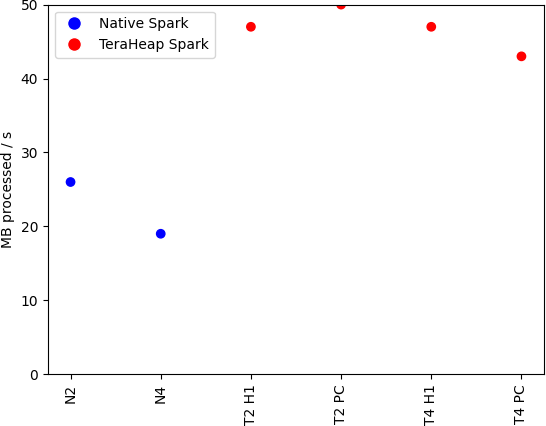
\includegraphics[width=\linewidth]{./fig/LOGR_64_THR.png}
    \caption{Logistic Regression 64 GB DRAM setup Native and TeraHeap
    throughput as the number of instances increases. Configurations
    starting with N denote a run with Native instances of Spark and
    with T with TeraHeap. H1 is a run with the memory budget
    configured to contain a bigger size for H1 than PageCache and PC
    the opposite. E.g. T2 PC is a run of 2 concurrent TeraHeap
    instances with exactly the same configuration.}
		\label{fig:logr_64_thr}
\end{figure}

\begin{figure}[thbp]
	\centering
        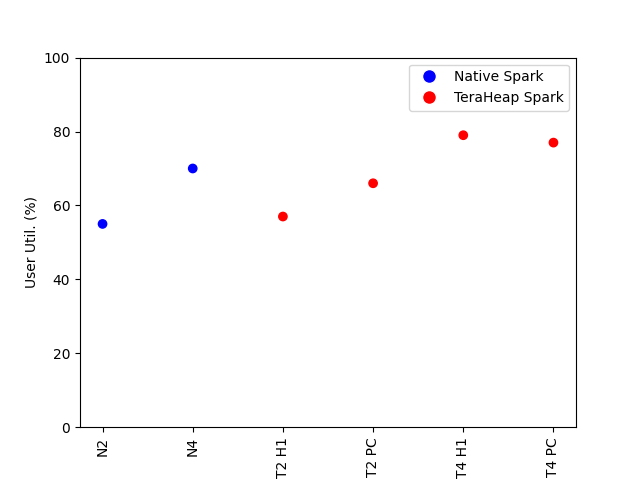
\includegraphics[width=\linewidth]{./fig/LINR_64_USR.png}
    \caption{Linear Regression 64 GB DRAM setup Native and TeraHeap
    User CPU utilization as the number of instances increases. Configurations
    starting with N denote a run with Native instances of Spark and
    with T with TeraHeap. H1 is a run with the memory budget
    configured to contain a bigger size for H1 than PageCache and PC
    the opposite. E.g. T2 PC is a run of 2 concurrent TeraHeap
    instances with exactly the same configuration.}
		\label{fig:linr_64_usr}
    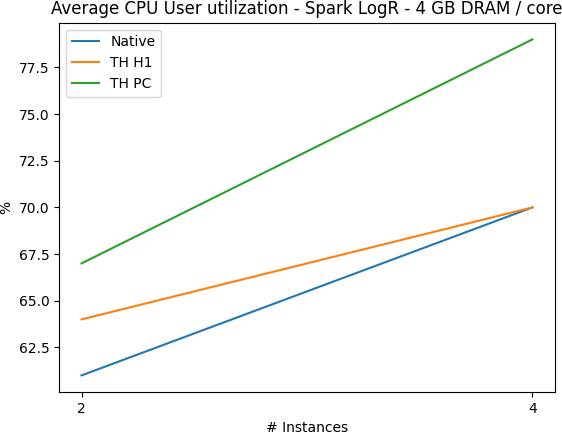
\includegraphics[width=\linewidth]{./fig/LOGR_64_USR.png}
    \caption{Logistic Regression 64 GB DRAM setup Native and TeraHeap
    User CPU utilization as the number of instances increases. Configurations
    starting with N denote a run with Native instances of Spark and
    with T with TeraHeap. H1 is a run with the memory budget
    configured to contain a bigger size for H1 than PageCache and PC
    the opposite. E.g. T2 PC is a run of 2 concurrent TeraHeap
    instances with exactly the same configuration.}
	   \label{fig:logr_64_usr}
\end{figure}

\begin{figure}[thbp]
	\centering
        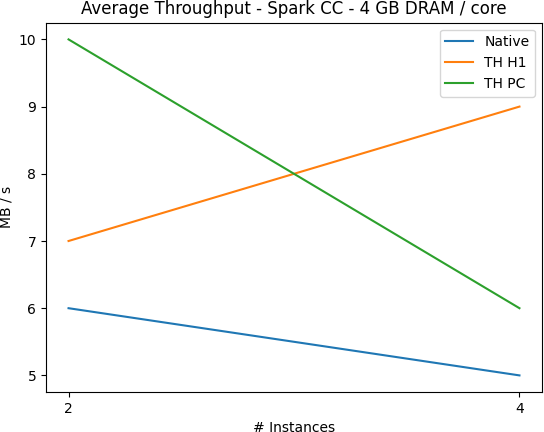
\includegraphics[width=\linewidth]{./fig/CC_64_THR.png}
    \caption{Connected Component 64 GB DRAM setup Native and TeraHeap
    throughput as the number of instances increases.Configurations
    starting with N denote a run with Native instances of Spark and
    with T with TeraHeap. H1 is a run with the memory budget
    configured to contain a bigger size for H1 than PageCache and PC
    the opposite. E.g. T2 PC is a run of 2 concurrent TeraHeap
    instances with exactly the same configuration. }
		\label{fig:cc_64_thr}
        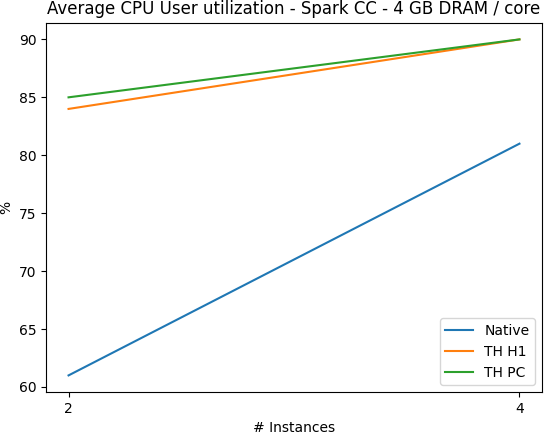
\includegraphics[width=\linewidth]{./fig/CC_64_USR.png}
    \caption{Connected Component 64 GB DRAM setup Native and TeraHeap
    User CPU utilization as the number of instances increases. Configurations
    starting with N denote a run with Native instances of Spark and
    with T with TeraHeap. H1 is a run with the memory budget
    configured to contain a bigger size for H1 than PageCache and PC
    the opposite. E.g. T2 PC is a run of 2 concurrent TeraHeap
    instances with exactly the same configuration.}
	\label{fig:cc_64_usr}
\end{figure}

\begin{figure}[thbp]
        \centering
        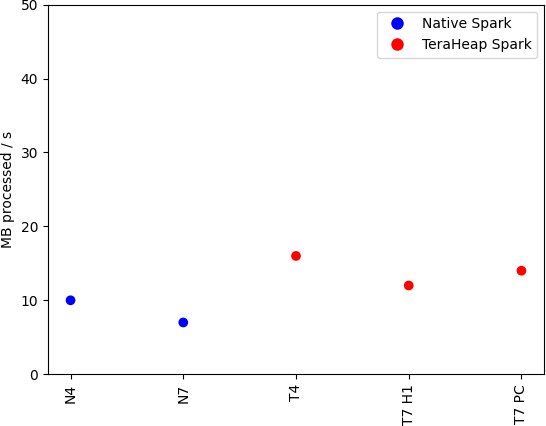
\includegraphics[width=\linewidth]{./fig/PR_256_THR.png}
    \caption{Page Rank 256 GB DRAM setup Native and TeraHeap
    throughput as the number of instances increases.Configurations
    starting with N denote a run with Native instances of Spark and
    with T with TeraHeap. H1 is a run with the memory budget
    configured to contain a bigger size for H1 than PageCache and PC
    the opposite. E.g. T2 PC is a run of 2 concurrent TeraHeap
    instances with exactly the same configuration. }
                \label{fig:pr_256_thr}
        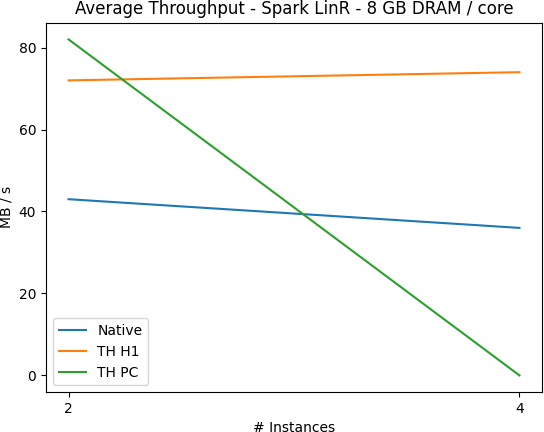
\includegraphics[width=\linewidth]{./fig/LINR_128_THR.png}
    \caption{Linear Regression 128 GB DRAM setup Native and TeraHeap
    throughput as the number of instances increases. Configurations
    starting with N denote a run with Native instances of Spark and
    with T with TeraHeap. H1 is a run with the memory budget
    configured to contain a bigger size for H1 than PageCache and PC
    the opposite. E.g. T2 PC is a run of 2 concurrent TeraHeap
    instances with exactly the same configuration.}
        \label{fig:linr_128_thr}
\end{figure}

\begin{figure}[thbp]
        \centering
        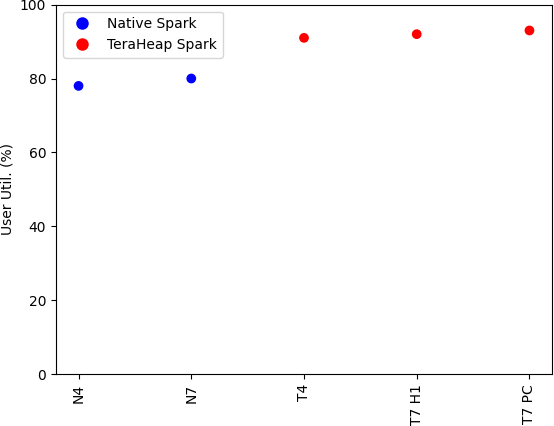
\includegraphics[width=\linewidth]{./fig/PR_256_USR.png}
    \caption{Page Rank 256 GB DRAM setup Native and TeraHeap
    User CPU utilization as the number of instances increases.Configurations
    starting with N denote a run with Native instances of Spark and
    with T with TeraHeap. H1 is a run with the memory budget
    configured to contain a bigger size for H1 than PageCache and PC
    the opposite. E.g. T2 PC is a run of 2 concurrent TeraHeap
    instances with exactly the same configuration. }
                \label{fig:pr_256_usr}
        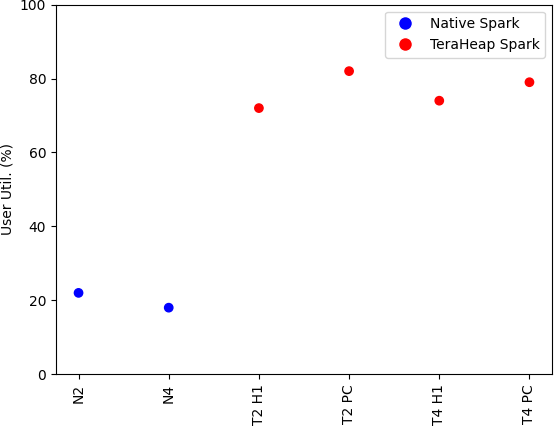
\includegraphics[width=\linewidth]{./fig/LINR_128_USR.png}
    \caption{Linear Regression 128 GB DRAM setup Native and TeraHeap
    User CPU utilization as the number of instances increases. Configurations
    starting with N denote a run with Native instances of Spark and
    with T with TeraHeap. H1 is a run with the memory budget
    configured to contain a bigger size for H1 than PageCache and PC
    the opposite. E.g. T2 PC is a run of 2 concurrent TeraHeap
    instances with exactly the same configuration.}
        \label{fig:linr_128_usr}
\end{figure}


The main goal for colocating tasks is to increase the CPU utilization and achieve better
throughput. CPU utilization is split to 2 parts. 
User utilization includes all CPU cycles that were executed in user-space threads.
It includes GC cycles, S/D cycles and mutator tasks except I/O.
System utilization includes all CPU cycles that were executed in kernel-space threads.
This includes I/O carried out by GC (TeraHeap) and mutator I/O.
Therefore we have to focus to User utilization which includes the effective CPU cycles done by the application.
By looking at figures \ref{fig:pr_64_thr}, \ref{fig:linr_64_thr},
\ref{fig:logr_64_thr} and \ref{fig:cc_64_thr} we see that Native
Spark's throughput decreases as the number of colocated
instances-executors increase in the server.
This is justified by GC and S/D that increase as instances increase and by the increased User utilization
(\ref{fig:pr_64_usr}, \ref{fig:linr_64_usr}, \ref{fig:logr_64_usr}, \ref{fig:cc_64_usr}).
TeraHeap achieves higher throughput than Native Spark and that is also justified by the increased User utilization.
Having higher user utilization and lower GC and S/D means that effective CPU utilization is really higher, since more
work is done by mutator threads.

\subsection{Single instance vs colocated instances}
When running colocated instances the goal is that the execution 
of all instances is close to the summary of execution of all instances run isolated.
As seen in tables, most of the times we are not even close. To achieve that
we need a scheduling policy to dynamically resize H1 and Page Cache based on runtime decisions.

\subsection{What
happens with monetary cost across different cloud platforms?}

\iffalse
\begin{table}[htbp]
  \centering
	\begin{subtable}[b]{0.45\linewidth}
  \caption{Page Rank synopsis table. Configurations starting
    with N denote a run with Native instances of Spark and with T with
    TeraHeap. H1 is a run with the memory budget configured to contain
    a bigger size for H1 than PageCache and PC the opposite.}
  \label{tab:pr_table}
        %\resizebox{19cm}{!}{
        \begin{tabular}{|c|c|c|c|c|c|c|c|c|c|c|c|c|}
      \hline
\textbf{Conf.} & \textbf{H1 Size/I} & \textbf{Memory/I} & \textbf{Total Mem.} & \textbf{\#I} & \textbf{Exec. Time} & \textbf{CPU Idle} & \textbf{Total MB Proc.} & \textbf{MB/s} & \textbf{MB/s/I} & \textbf{Cost AWS \$} & \textbf{Cost GCP \$} & \textbf{Cost Azure \$} \\
        \hline
    N2 - small & 22 & 28 & 64 & 2 & 3563 & 29 & 16980 & 5 & 2 & 0.6 & 0.58 & 0.67 \\
    N4 - small & 11 & 14 & 64 & 4 & 8195 & 11 & 33960 & 4 & 1 & 1.8 & 1.74 & 2.01 \\
    T2 H1 – small & 22 & 28 & 64 & 2 & 2545 & 7 & 16980 & 7 & 3 & 0.6 & 0.58 & 0.67 \\
    T2 PC – small & 11 & 28 & 64 & 2 & 2385 & 9 & 16980 & 7 & 4 & 0.6 & 0.58 & 0.67 \\
    T4 H1 – small & 11 & 14 & 64 & 4 & 5554 & 1 & 33960 & 6 & 2 & 1.2 & 1.16 & 1.34 \\
    T4 PC – small & 6 & 14 & 64 & 4 & 5880 & 1 & 33960 & 6 & 2 & 1.2 & 1.16 & 1.34 \\
    N8 – small & 4 & 7 & 64 & 8 & OOM & ** & 0 & 0 & 0 & *** & *** & *** \\
    T8 – small & 4 & 7 & 64 & 8 & 12305 & 0 & 67920 & 6 & 1 & 2.4 & 2.32 & 2.68 \\
    N4 - big & 44 & 60 & 256 & 4 & 13542 & 15 & 135872 & 10 & 3 & 6.4 & *** & *** \\
    T4 – big & 48 & 60 & 256 & 4 & 9284 & 5 & 135782 & 16 & 4 \\      
	\hline
     \end{tabular}%
        %}
\end{subtable}

	\begin{subtable}[b]{0.45\linewidth}
  \caption{Linear Regression synopsis table. Configurations starting
    with N denote a run with Native instances of Spark and with T with
    TeraHeap. H1 is a run with the memory budget configured to contain
    a bigger size for H1 than PageCache and PC the opposite.}
  \label{tab:linr_table}
        %\resizebox{19cm}{!}{
        \begin{tabular}{|c|c|c|c|c|c|c|c|c|c|c|c|c|}
      \hline
\textbf{Conf.} & \textbf{H1 Size/I} & \textbf{Memory/I} & \textbf{Total Mem.} & \textbf{\#I} & \textbf{Exec. Time} & \textbf{CPU Idle} & \textbf{Total MB Proc.} & \textbf{MB/s} & \textbf{MB/s/I} & \textbf{Cost AWS \$} & \textbf{Cost GCP \$} & \textbf{Cost Azure \$} \\
	\hline 
      N2 & 22 & 28 & 64 & 2 & 3745 & 20 & 134896 & 37 & 18 & 0.6 & 0.58 & 0.67 \\ 
      N4 & 11 & 14 & 64 & 4 & 13874 & 7 & 269792 & 20 & 5 & 2.4 & 2.32 & 2.01 \\
      T2 H1 & 22 & 28 & 64 & 2 & 2891 & 19 & 134896 & 48 & 24 & 0.6 & 0.58 & 0.67 \\
      T2 PC & 11 & 28 & 64 & 2 & 2747 & 18 & 134896 & 49 & 25 & 0.6 & 0.58 & 0.67 \\
      T4 H1 & 11 & 14 & 64 & 4 & 6075 & 2 & 269792 & 44 & 11 & 1.2 & 1.16 & 1.34 \\
      T4 PC & 6 & 14 & 64 & 4 & 6176 & 3 & 269792 & 44 & 11 & 1.2 & 1.16 & 1.34 \\ 
      \hline
     \end{tabular}%
	%}
\end{subtable}
	\vspace{1em}
\end{table}
\fi
%\iffalse
%\begin{center}%[htbp]
 %   \centering
  %  \caption{Page Rank synopsis table}
\begin{table*}
\resizebox{\textwidth}{!}{
\begin{tabular}{|c|c|c|c|c|c|c|c|c|c|c|c|c|c|c|c|c|}
		%\begin{tabularx}{\linewidth}{*{17}{X}}
	    \hline
        \multirow{2}{*}{Configuration} & H1       & \multirow{2}{*}{Mem / I} & Total & \multirow{2}{*}{\#I} & Exec. & User  & System & I/O  & CPU  & Total MB  & \multirow{2}{*}{MB/s} & \multirow{2}{*}{MB/s/I} & Cost   & Cost   & Cost \\
                                       & Size / I &                          & memory &                     & Time  & util. & util.  & Wait & Idle & Processed &                       &                         & AWS \$ & GCP \$ & Azure \$ \\
        \hline
        \hline
        N2-small – single & 22 & 28 & 64 & 1 & 1762 & 32 & 2 & 1 & 65 & 8490 & 5 & 5 & 0.6 & 0.58 & 0.67 \\
        N2 - small & 22 & 28 & 64 & 2 & 3563 & 66 & 5 & 2 & 27 & 16980 & 5 & 2 & 0.6 & 0.58 & 0.67 \\
        N4 – small – single & 11 & 14 & 64 & 1 & 1783 & 29 & 2 & 1 & 68 & 8490 & 5 & 5 & 0.6 & 0.58 & 0.67 \\
        N4 - small & 11 & 14 & 64 & 4 & 8195 & 84 & 6 & 2 & 8 & 33960 & 4 & 1 & 1.8 & 1.74 & 2.01 \\
        N8 – small & 4 & 7 & 64 & 8 & OOM & 0 & 0 & 0 & ** & 0 & 0 & 0 & *** & *** & *** \\
        T2 H1- small – single & 22 & 28 & 64 & 1 & 1146 & 46 & 2 & 1 & 51 & 8490 & 7 & 7 & 0.6 & 0.58 & 0.67 \\
        T2 H1 – small & 22 & 28 & 64 & 2 & 2545 & 89 & 4 & 1 & 6 & 16980 & 7 & 3 & 0.6 & 0.58 & 0.67 \\
        T2 PC- small – single & 11 & 28 & 64 & 1 & 966 & 45 & 2 & 1 & 52 & 8490 & 9 & 9 & 0.6 & 0.58 & 0.67 \\
        T2 PC – small & 11 & 28 & 64 & 2 & 2385 & 87 & 4 & 0 & 9 & 16980 & 7 & 4 & 0.6 & 0.58 & 0.67 \\
        T4 H1 – small – single & 11 & 14 & 64 & 1 & 984 & 43 & 3 & 1 & 53 & 8490 & 9 & 9 & 0.6 & 0.58 & 0.67 \\
        T4 H1 – small & 11 & 14 & 64 & 4 & 5554 & 94 & 5 & 0 & 1 & 33960 & 6 & 2 & 1.2 & 1.16 & 1.34 \\
        T4 PC – small – single & 6 & 14 & 64 & 1 & 922 & 42 & 2 & 2 & 54 & 8490 & 9 & 9 & 0.6 & 0.58 & 0.67 \\
        T4 PC – small & 6 & 14 & 64 & 4 & 5880 & 94 & 5 & 0 & 1 & 33960 & 6 & 2 & 1.2 & 1.16 & 1.34 \\
        T8 – small – single & 4 & 7 & 64 & 1 & 1037 & 39 & 2 & 1 & 58 & 8490 & 8 & 8 & 0.6 & 0.58 & 0.67 \\
        T8 – small & 4 & 7 & 64 & 8 & 12305 & 95 & 5 & 0 & 0 & 67920 & 6 & 1 & 2.4 & 2.32 & 2.68 \\
        N4 - big & 48 & 60 & 256 & 4 & 13542 & 78 & 7 & 7 & 8 & 135872 & 10 & 3 & 6.4 & *** & *** \\
        T4 – big & 48 & 60 & 256 & 4 & 9284 & 91 & 8 & 1 & 1 & 135782 & 16 & 4 & 1.8 & *** & *** \\
        N7 – big & 27 & 34 & 256 & 7 & 32763 & 80 & 8 & 12 & 0 & 237776 & 7 & 1 & 14.4 & *** & *** \\
        T7 H1 – big & 27 & 34 & 256 & 7 & 19443 & 92 & 7 & 1 & 0 & 237776 & 12 & 2 & 9.6 & *** & *** \\
        T7 PC – big & 14 & 34 & 256 & 7 & 16485 & 93 & 7 & 1 & 0 & 237776 & 14 & 2 & 8 & *** & *** \\
        \hline
	\bottomrule
\end{tabular}
}
\end{table*}
%	\label{tab:pr_table}
%\end{center}
%\fi
\iffalse
\begin{table}[t!]
  \centering
  \caption{Logistic Regression synopsis table. Configurations starting
    with N denote a run with Native instances of Spark and with T with
    TeraHeap. H1 is a run with the memory budget configured to contain
    a bigger size for H1 than PageCache and PC the opposite.}
  \label{tab:logr_table}
	\resizebox{19cm}{!}{
	\begin{tabular}{|c|c|c|c|c|c|c|c|c|c|c|c|c|}
      \hline
\textbf{Conf.} & \textbf{H1 Size/I} & \textbf{Memory/I} & \textbf{Total Mem.} & \textbf{\#I} & \textbf{Exec. Time} & \textbf{CPU Idle} & \textbf{Total MB Proc.} & \textbf{MB/s} & \textbf{MB/s/I} & \textbf{Cost AWS \$} & \textbf{Cost GCP \$} & \textbf{Cost Azure \$} \\
      \hline
      N2 & 22 & 28 & 64 & 2 & 5127 & 18 & 133348 & 26 & 13 & 1.2 & 1.16 & 0.67 \\
      N4 & 11 & 14 & 64 & 4 & 13730 & 7 & 266696 & 19 & 5 & 2.4 & 2.32 & 2.68 \\
      T2 H1 & 22 & 28 & 64 & 2 & 2861 & 18 & 133348 & 47 & 24 & 0.6 & 0.58 & 0.67 \\
      T2 PC & 11 & 28 & 64 & 2 & 2683 & 18 & 133348 & 50 & 25 & 0.6 & 0.58 & 0.67 \\
      T4 H1 & 10 & 14 & 64 & 4 & 5712 & 2 & 266696 & 47 & 12 & 1.2 & 1.16 & 1.34 \\
      T4 PC & 6 & 14 & 64 & 4 & 6138 & 2 & 266696 & 43 & 10 & 1.2 & 1.16 & 1.34 \\
      \hline
     \end{tabular}%
	}
\end{table}

\begin{table}[t!]
  \centering
  \caption{Connected Component synopsis table. Configurations starting
    with N denote a run with Native instances of Spark and with T with
    TeraHeap. H1 is a run with the memory budget configured to contain
    a bigger size for H1 than PageCache and PC the opposite.}
  \label{tab:cc_table}
        \resizebox{19cm}{!}{
        \begin{tabular}{|c|c|c|c|c|c|c|c|c|c|c|c|c|}
      \hline
\textbf{Conf.} & \textbf{H1 Size/I} & \textbf{Memory/I} & \textbf{Total Mem.} & \textbf{\#I} & \textbf{Exec. Time} & \textbf{CPU Idle} & \textbf{Total MB Proc.} & \textbf{MB/s} & \textbf{MB/s/I} & \textbf{Cost AWS \$} & \textbf{Cost GCP \$} & \textbf{Cost Azure \$} \\
	\hline
      N2 & 22 & 28 & 64 & 2 & 2958 & 26 & 16980 & 6 & 3 & 0.6 & 0.58 & 0.67 \\
      N4 & 11 & 14 & 64 & 4 & 7231 & 7 & 33960 & 5 & 3 & 1.8 & 1.74 & 2.01 \\
      T2 H1 & 22 & 28 & 64 & 2 & 2526 & 5 & 16980 & 7 & 4 & 0.6 & 0.58 & 0.67 \\
      T2 PC & 11 & 28 & 64 & 2 & 2519 & 7 & 16980 & 7 & 4 & 0.6 & 0.58 & 0.67 \\
      T4 H1 & 11 & 14 & 64 & 4 & 5439 & 3 & 33960 & 6 & 3 & 1.2 & 0.58 & 0.67 \\
      T4 PC & 6 & 14 & 64 & 4 & 5487 & 2 & 33960 & 6 & 3 & 1.2 & 1.16 & 1.34 \\
      \hline
     \end{tabular}%
	}
\end{table}
\fi

Tables \ref{tab:pr_table}, \ref{tab:linr_table}, \ref{tab:logr_table}
and \ref{tab:cc_table} show 
Amazon Web Services Cloud (EC2), GCP (Google Cloud Platform) and Microsoft Azure costs of deploying multiple instances of Spark
using both techniques. 
We witness that all providers offer a similar cost for identical machines to our server. 
As seen by the tables, taking into account that we have an hourly cost,
TeraHeap could be used for running colocated Spark and Giraph workloads
and save money. Reducing the GC and S/D makes a huge difference in the execution time
and therefore running with TeraHeap decreases the hours needed to rent the machines.


\section{Future Work}

While this analysis shows promising results and provides a methodology for understanding
throughput for big data analytics workloads on Spark and Giraph
clusters, there are several avenues for future work to use it on and
improve performance and scalability. 

Firstly, one potential direction for future work is to investigate the
use of other types of storage mediums such as the hybrid NVM. This
medium could improve the performance of Big data analytics further by
combining the advantages of memory and storage.

Secondly, another area for future work is to develop techniques for
dynamically adjusting the heap offloading decisions based on workload
characteristics and resource availability. For example, the offloading
decision can be based on the size of the input data or the
availability of DRAM capacity in the cluster. Such techniques can help
maximize the performance gains achieved by offloading while minimizing
the cost of offloading.

Thirdly, an interesting direction for future work is to explore the
use of heap offloading in environments where Spark-Giraph clusters are
deployed across multiple machines using RDMA to achieve communication
between the different machines. This can help utilize the DRAM, CPU
and storage availability in more than one machine and provide a more
cost-effective solution for big data processing.


\section{Conclusions}

In this paper, we conducted an analysis of throughput for managed big data analytics frameworks
using Apache Spark and Giraph under workload co-location. We investigated if reducing GC and S/D for managed big data frameworks can improve application throughput by using TeraHeap. We conducted our experiments under 2 different memory-per-core
scnarios, 4 and 8 GB / core. 4 GB / core is the current trend and 8 GB / core is a possible future trend. 
We showed how someone can adjust the DRAM capacity to create different memory/core setups.
Then for simplicity we divided total DRAM capacity to 2,4 and 8 even memory budgets. We used each budget to run each instance isolated with Native Spark and Giraph and Spark and Giraph using TH to study the execution breakdown.
Then we run experiments with 2,4 and 8 co-located instances using the above budgets for each instance. We ran 4 Spark workloads (PR, LinR, LogR and CC) in the 4 GB / core scenario and 1 Spark workload (LinR) and 2 Giraph workloads (PR, CDLP) in the 8 GB / core scenario. We ran Giraph under 8 GB / core because it is more memory intensive than Spark. We report interference with single instance, execution breakdown (GC, S/D, I/O), user CPU utilization and average throughput.

Our experimental results showed that reducing GC and S/D for both Spark and Giraph reduces execution time and increases the effective CPU utilization by the applications threads. 
For Spark under 4 GB memory / core reducing GC and S/D increases average server throughput by up to 66\% against native Spark.
For Spark under 8 GB memory / core reducing GC and S/D increases up to 77\% more average throughput against Native Spark.
For Giraph under 8 GB memory / core reducing GC and S/D increases up to 13\% more average throughput against Native Giraph. 

Overall, our analysis showed that high CPU utilization does not always mean that useful work is done by the CPU. Specificaly for managed
big data frameworks like Spark and Giraph a lot of CPU cycles are wasted on GC and S/D and even increasing H1 does not guarantee optimal execution.


%-------------------------------------------------------------------------------
\bibliographystyle{plain}
\bibliography{paper}

%%%%%%%%%%%%%%%%%%%%%%%%%%%%%%%%%%%%%%%%%%%%%%%%%%%%%%%%%%%%%%%%%%%%%%%%%%%%%%%%
\end{document}
%%%%%%%%%%%%%%%%%%%%%%%%%%%%%%%%%%%%%%%%%%%%%%%%%%%%%%%%%%%%%%%%%%%%%%%%%%%%%%%%
